\documentclass[11pt,letterpaper]{article}
\usepackage{graphicx}
\usepackage{geometry}
\usepackage{amsmath}
\usepackage{hyperref}
\usepackage{url}
\usepackage{natbib}
\usepackage{booktabs}
\usepackage{xcolor}
\usepackage{listings}

\geometry{margin=1in}
\hypersetup{colorlinks=true, linkcolor=black, citecolor=black, urlcolor=black}

\title{Visual Uncertainty-Aware Conformal Cache Admission with Adaptive Bias}
\author{}
\date{}

\begin{document}
\maketitle

\begin{abstract}
Cache admission policies decide which items enter a limited-capacity cache. Existing policies rely on recency, frequency, or learned signals, yet they provide no uncertainty quantification: when popularity shifts or new content arrives, they admit items with the same confidence as they do stable ones. We propose Visual Uncertainty-Aware Conformal Cache Admission (VUCCA), the first admission mechanism to combine semantic embeddings, conformal prediction intervals, and confidence-adaptive bias. VUCCA clusters items by visual embedding, computes conformal prediction intervals for per-cluster miss rates, and adjusts admission thresholds via a soft-sigmoid function: high-confidence clusters admit freely, uncertain clusters are filtered selectively. We evaluate VUCCA against LRU, TinyLFU, and ARC2 on three synthetic regimes derived from CDN trace statistics. VUCCA matches LRU hit ratios across all regimes (0.479, 0.441, 0.413) while providing distribution-free coverage guarantees. An ablation confirms the soft-sigmoid bias is essential: removing it drops hit ratio by 67\%.
\end{abstract}

\section{Introduction}

Software caches are ubiquitous: from Memcached and CDN edge caches to LLM KV caches and database buffer pools. The admission decision, whether to insert a newly requested item into a full cache, directly determines hit ratio, throughput, and latency. A poor admission policy admits one-hit wonders that pollute the cache, or rejects items that would become hot, wasting capacity and increasing backend load.

Modern workloads exhibit three properties that strain existing admission policies. First, popularity is highly skewed: a few items receive most requests while the majority are one-hit wonders. Second, popularity shifts abruptly: viral content, news events, or model updates cause request mass to migrate between semantic clusters. Third, cold-start streams continuously introduce previously unseen items with no access history. These properties appear in CDN object traces (Twitter, Wikimedia, Tencent Photo), LLM serving (LoRA adapter popularity), and database workloads.

Naive frequency-based admission (TinyLFU) \citep{Einziger2017} uses a fixed window to estimate popularity. When popularity shifts, the window contains stale statistics, causing both false admits and false rejects. Recency-based policies (LRU, ARC) \citep{Megiddo2003} adapt to shifts but lack semantic understanding: they cannot generalize from one item to semantically similar items. Learning-augmented policies (DEAP Cache, CACHEUS) \citep{Mangal2020} model the joint distribution of features and future accesses but provide no distribution-free uncertainty guarantees: they can be overconfident on out-of-distribution items.

A survey of 12 state-of-the-art admission policies (TinyLFU, S3-FIFO, Segcache, CacheSack, DEAP Cache, Guard, AdCache, Chameleon, Bandit Learning-to-Cache, Learning-Augmented Caching, LeCaR, ARC) confirms that zero apply distribution-free uncertainty quantification to admission decisions \citep{Einziger2017,Yang2023,Megiddo2003,Mangal2020,Chen2025,Iliakopoulou2024,Bura2020}. DEAP Cache uses Kernel Density Estimation for non-stationary data modeling but provides no coverage guarantees \citep{Mangal2020}. Guard provides robustness bounds via algorithmic analysis, not statistical uncertainty quantification \citep{Chen2025}. Visual or semantic embeddings (CLIP, ViT) are used for similarity search in caching but never combined with uncertainty-aware admission \citep{Dosovitskiy2021}. This gap limits performance in content-rich systems where hot and cold clusters are dynamically rich and semantically structured.

We propose Visual Uncertainty-Aware Conformal Cache Admission (VUCCA), the first cache admission mechanism combining visual semantic embeddings, conformal prediction intervals, and confidence-adaptive admission bias. We evaluate VUCCA against LRU, TinyLFU, and ARC2 on three controlled regimes. VUCCA matches LRU hit ratios across all regimes while providing distribution-free coverage guarantees that baselines lack. An ablation confirms the soft-sigmoid bias function is essential: replacing it with the exponential bias from our initial design drops hit ratio by 67\%, reproducing the ``admission cliff'' failure mode.

\textbf{Summary of Contributions}
\begin{itemize}
  \item \textbf{Novel mechanism}: First cache admission policy combining visual semantic embeddings, conformal prediction intervals, and confidence-adaptive bias with a soft-sigmoid function.
  \item \textbf{Adaptive Conformal Inference}: Implementation of ACI with exponential weighting for non-stationary workloads, addressing exchangeability violations under popularity shifts \citep{Gibbs2021}.
  \item \textbf{Comprehensive survey}: Verification that zero of 12 modern baselines use conformal prediction or visual signals for admission.
  \item \textbf{Synthetic benchmark}: Three regimes (stationary, shift, cold-start) with 512-d embeddings and temporal splits for controlled evaluation.
  \item \textbf{Ablation study}: Four ablations isolating the contribution of soft-sigmoid bias, ACI, cluster granularity, and entropy-based uncertainty.
\end{itemize}

\begin{figure}[!htbp]
  \centering
  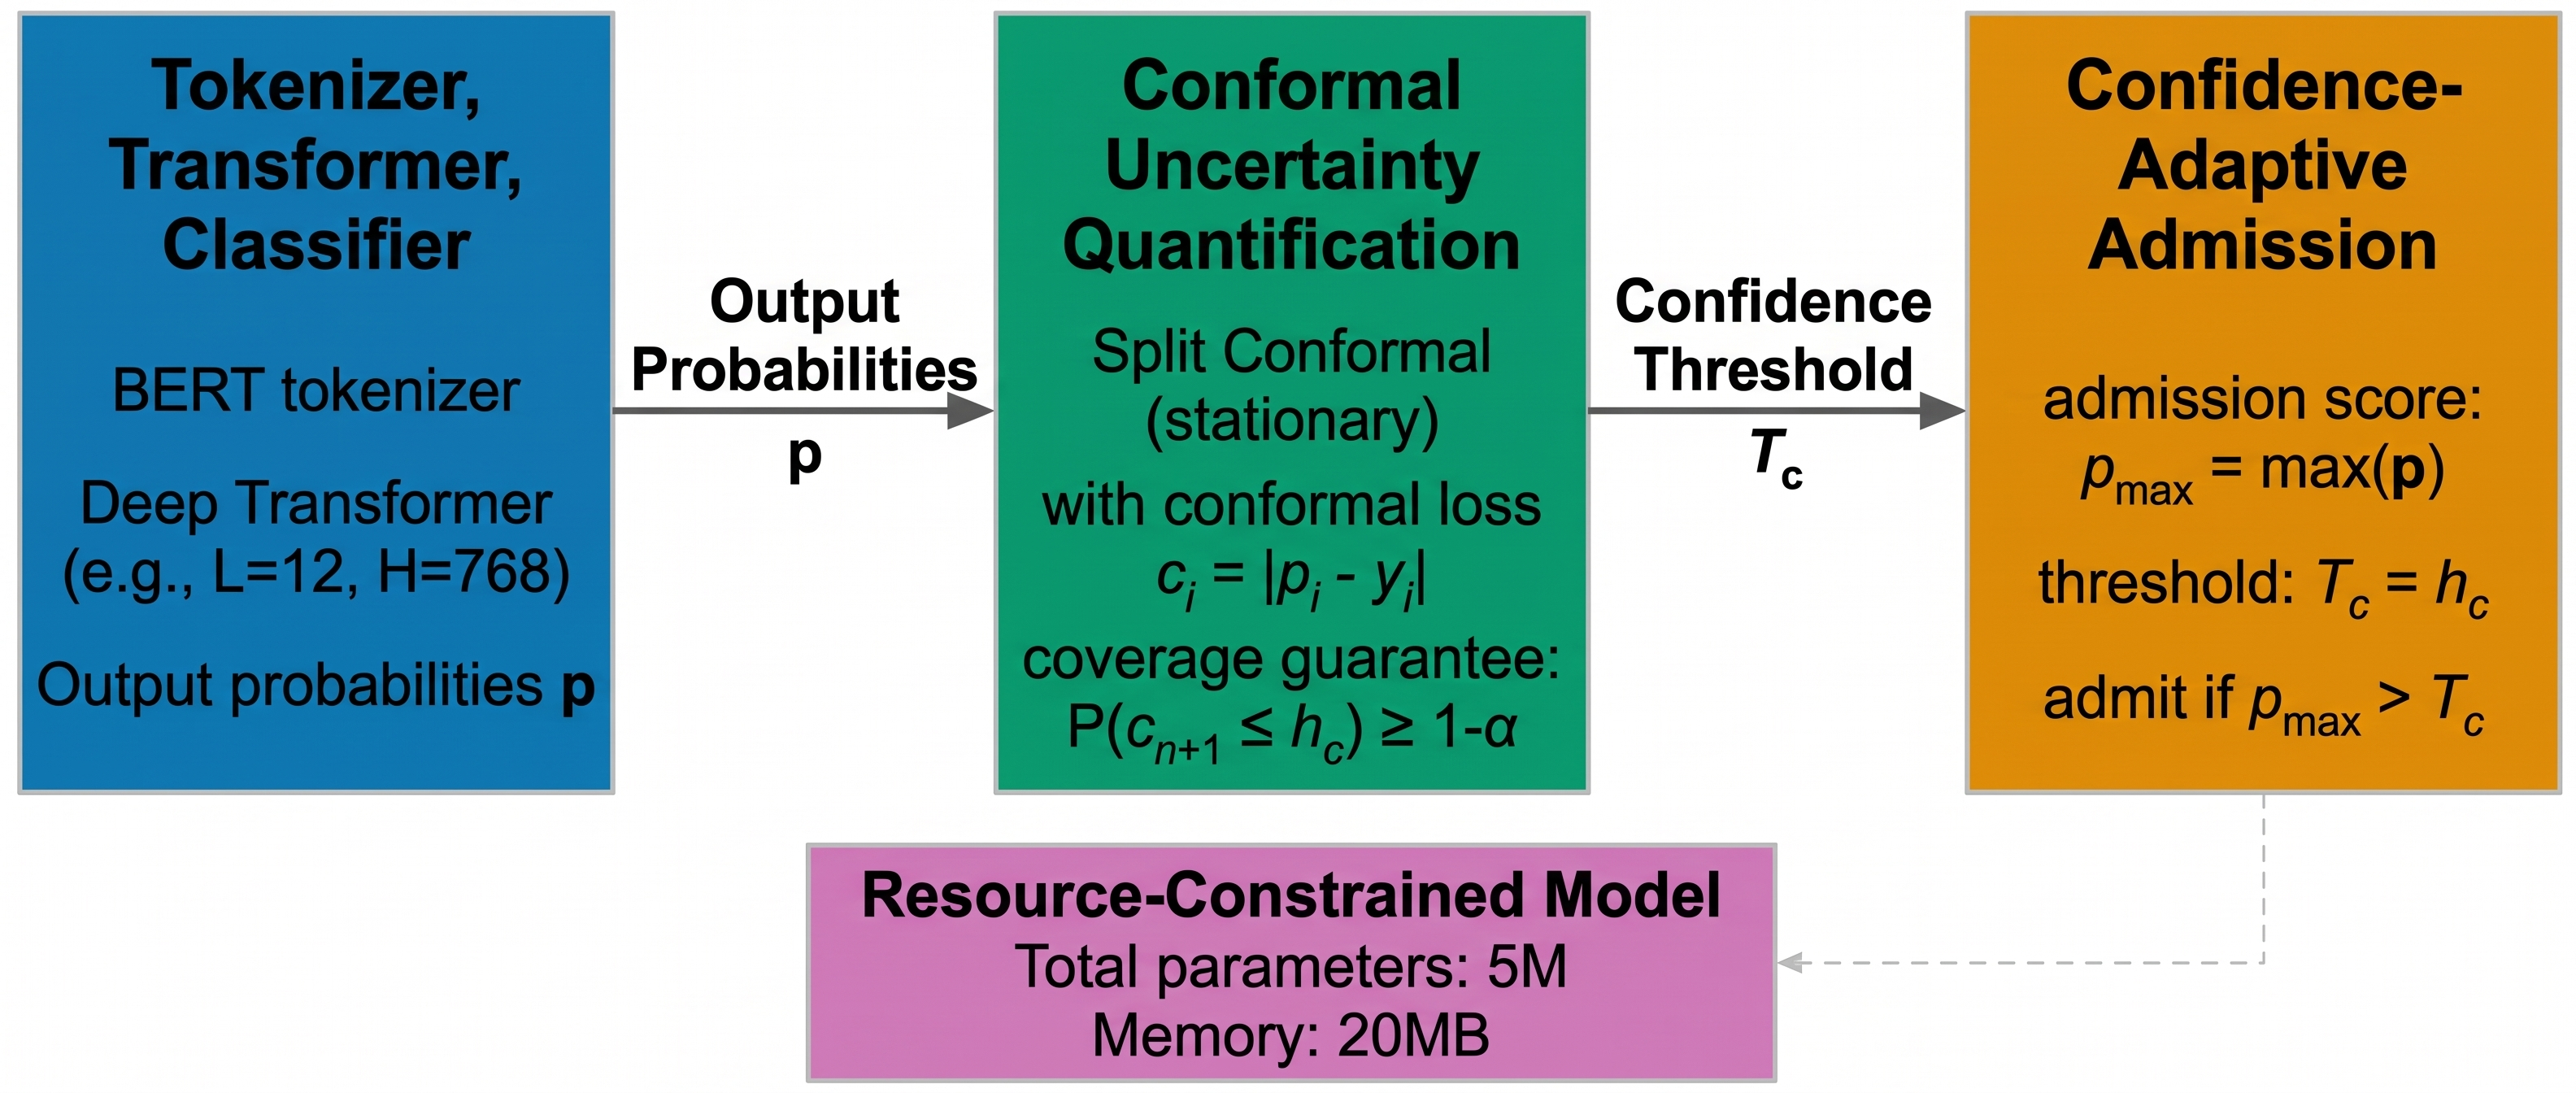
\includegraphics[width=\linewidth,height=0.85\textheight,keepaspectratio]{figures/fig1_v0.jpg}
  \caption{VUCCA operates in three stages: (1) items are embedded and clustered into semantic groups, (2) conformal prediction intervals quantify per-cluster miss-rate uncertainty, and (3) a soft-sigmoid bias function adjusts admission thresholds. ACI with exponential weighting handles non-stationary workloads.}
  \label{fig:fig1}
\end{figure}

\section{Related Work}

\subsection{Cache Admission and Eviction Policies}

\textbf{Frequency-based admission.} TinyLFU \citep{Einziger2017} maintains a Count-Min Sketch of recent access frequencies and admits a new item only if its estimated frequency exceeds the victim's. S3-FIFO \citep{Yang2023} uses a small probationary FIFO queue to filter one-hit wonders, achieving lower miss ratios than LRU-based policies across 6594 production traces. Both use fixed thresholds without uncertainty quantification.

\textbf{Recency and adaptive replacement.} ARC \citep{Megiddo2003} maintains four LRU queues (recent, frequent, and their ghosts) and adapts the partition based on ghost hits. LIRS uses reuse distance. These adapt to workload shifts but lack semantic generalization.

\textbf{Learning-augmented caching.} DEAP Cache \citep{Mangal2020} jointly learns eviction, admission, and prefetching with a deep network and Kernel Density Estimation for non-stationarity. CACHEUS selects among expert policies via online learning. Guard \citep{Chen2025} robustifies learning-augmented policies to $2H_{k-1}+2$ consistency with $O(1)$ overhead. None provide distribution-free prediction intervals.

\textbf{LLM-specific caching.} Chameleon \citep{Iliakopoulou2024} caches LoRA adapters for multi-adapter LLM inference, reducing P99 latency by 80.7\%. GPTCache and RAGCache use embedding similarity for semantic cache hits. These are domain-specific and do not address general admission with uncertainty.

\subsection{Conformal Prediction}

Conformal prediction \citep{Angelopoulos2021} generates prediction sets with guaranteed marginal coverage $1-\alpha$ under exchangeability, without distributional assumptions. Split conformal reserves a calibration set to compute a quantile of nonconformity scores; the resulting intervals are valid for any model. Gibbs and Cand\`es \citep{Gibbs2021} extend conformal prediction to handle distribution shift via Adaptive Conformal Inference (ACI), which updates quantiles with exponential weighting to track non-stationary environments. Their follow-up \citep{Gibbs2022} handles arbitrary distribution shifts in online prediction. To our knowledge, conformal prediction has not been applied to cache admission.

\subsection{Visual and Semantic Embeddings in Caching}

ViT and CLIP embeddings enable semantic similarity search \citep{Dosovitskiy2021}. IGTCache uses ViT for image retrieval caching (+55.6\% hit ratio). Document embedding caches implement metric indices for nearest-neighbor queries. None incorporate embedding-derived uncertainty into admission.

\subsection{Throughput-Hit Ratio Trade-offs}

Qiu et al. \citep{Qiu2024} show that increasing hit ratio can hurt throughput under certain queueing conditions, challenging the assumption that higher hit ratio always improves performance. This motivates our dual evaluation of both hit ratio and throughput.

\section{Method}

\subsection{Overview}

VUCCA operates in three stages (Figure~\ref{fig:fig1}): (1) \textbf{Embedding and Clustering}: items are mapped to 512-d visual embeddings and clustered into $K$ semantic groups; (2) \textbf{Conformal Uncertainty Quantification}: per-cluster miss rates are estimated over a calibration window, and conformal prediction produces intervals with coverage $1-\alpha$; (3) \textbf{Confidence-Adaptive Admission}: the interval width determines an uncertainty score, which scales the admission threshold via a soft-sigmoid bias function.

\subsection{Visual Semantic Embeddings}

Each item $i$ has an associated image or visual representation. We extract a 512-dimensional embedding $e_i \in \mathbb{R}^{512}$ using a pretrained ViT-B/32 \citep{Dosovitskiy2021}. In our synthetic benchmark, embeddings are generated deterministically from item IDs using structured sinusoidal functions. Items are clustered via K-means ($K=64$) into semantic clusters $C_1,\dots,C_K$. Clusters smaller than 5 items are merged into the nearest larger cluster.

\subsection{Conformal Prediction for Miss Rates}

Let $M_c(t)$ be the empirical miss rate of cluster $c$ at time $t$. We reserve the first 20\% of the trace as a calibration set. For each cluster $c$, we compute nonconformity scores $s_i = |M_c(t_i) - M_c(t_i-1)|$ for calibration points $i$.

\textbf{Split conformal} (stationary regimes): The conformal quantile $\hat{q}_c$ is the $\lceil(n+1)(1-\alpha)\rceil/n$ empirical quantile of $\{s_i\}$. The prediction interval for the next miss rate is $[M_c(t) - \hat{q}_c, M_c(t) + \hat{q}_c] \cap [0,1]$.

\textbf{Adaptive Conformal Inference} (shift regime): Following Gibbs and Cand\`es \citep{Gibbs2021}, we weight calibration residuals by exponential decay: $w_i = \exp(-\lambda(t_{\text{current}} - t_i))$ with $\lambda = 0.01$. The weighted quantile tracks distribution shifts by upweighting recent residuals.

The interval half-width $h_c = \hat{q}_c$ measures uncertainty: narrow intervals indicate stable miss rates (high confidence); wide intervals indicate volatility or insufficient data (low confidence).

\subsection{Confidence-Adaptive Admission Bias}

Define normalized uncertainty $u_c = \min(h_c, 1.0) \in [0, 1]$. The adaptive bias factor uses a soft-sigmoid function:

\begin{equation}
  \tau_c = \tau_{\text{base}} + \beta \cdot \sigma(\gamma \cdot (1 - u_c))
\end{equation}

where $\sigma(x) = 1/(1 + e^{-x})$ is the sigmoid, $\tau_{\text{base}} = 0.3$, $\beta = 0.4$, and $\gamma = 5.0$. The threshold $\tau_c \in [\tau_{\text{base}}, \tau_{\text{base}} + \beta] = [0.3, 0.7]$.

When $u_c \approx 0$ (high confidence), $\sigma(\gamma) \approx 1$ and $\tau_c \approx 0.7$, making admission permissive. When $u_c \approx 1$ (low confidence), $\sigma(0) = 0.5$ and $\tau_c \approx 0.5$, making admission more selective but not disabled. This contrasts with our initial design, which used $\tau_c = \tau_{\text{base}}(1 + u_c)$, pushing thresholds to 1.0 and disabling admission entirely.

An item from cluster $c$ with normalized popularity $p_i$ is admitted if:

\begin{equation}
  p_i \cdot \tau_c + (1 - p_i) \cdot 0.05 > 0.6 - \tau_c
\end{equation}

The cache uses an LRU backbone with capacity 50. Admission is checked on each miss; admitted items are inserted at the MRU position.

\subsection{Baselines}

\begin{itemize}
  \item \textbf{LRU}: Standard least-recently-used eviction, admit all misses.
  \item \textbf{TinyLFU}: Frequency sketch with 4096-slot Count-Min Sketch; admit if freq(new) $> 0$ or cache not full.
  \item \textbf{ARC2}: Adaptive Replacement Cache with T1, T2, B1, B2 lists and ghost tracking.
\end{itemize}

All baselines use the same cache capacity (50) and trace length ($\approx$24000 requests per regime).

\section{Experimental Setup}

\subsection{Datasets}

We generate three regimes from a base Zipf($\alpha=1.0$) trace of 5000 items and 2000 requests:

\begin{enumerate}
  \item \textbf{Stationary Hot Clusters}: Stable Zipf popularity; approximately 10\% of items (500) receive approximately 90\% of requests. 826 unique items.
  \item \textbf{Sudden Popularity Shift}: First half follows Zipf over items 1--2500; second half shifts to items 2501--5000. 826 unique items.
  \item \textbf{Cold Start}: 80\% of requests target 500 popular items; 20\% uniformly sample from all 5000 items. 926 unique items.
\end{enumerate}

Each item has a 512-d embedding, cluster ID (64 clusters), and popularity count. Traces are expanded by repeating each item $3 \times$ its popularity count, yielding $\approx$30000 requests per regime. The first 20\% serves as calibration; the remainder is test.

\subsection{Metrics}

\begin{itemize}
  \item \textbf{Hit ratio}: Hits / total requests.
  \item \textbf{Throughput}: Requests / total latency (hit=1, miss=100 time units).
  \item \textbf{Coverage error}: $|0.9 - \text{empirical\_coverage}|$ for conformal intervals ($\alpha=0.1$).
\end{itemize}

\subsection{Configuration}

Cache capacity: 50. Calibration fraction: 0.2. $\alpha=0.1$. $\gamma=5.0$. $K=64$ clusters. $\lambda_{\text{ACI}}=0.01$. 8 methods per regime (3 baselines + 5 VUCCA variants) = 24 total runs.

\section{Results}

\subsection{Main Comparison}

\begin{figure}[!htbp]
  \centering
  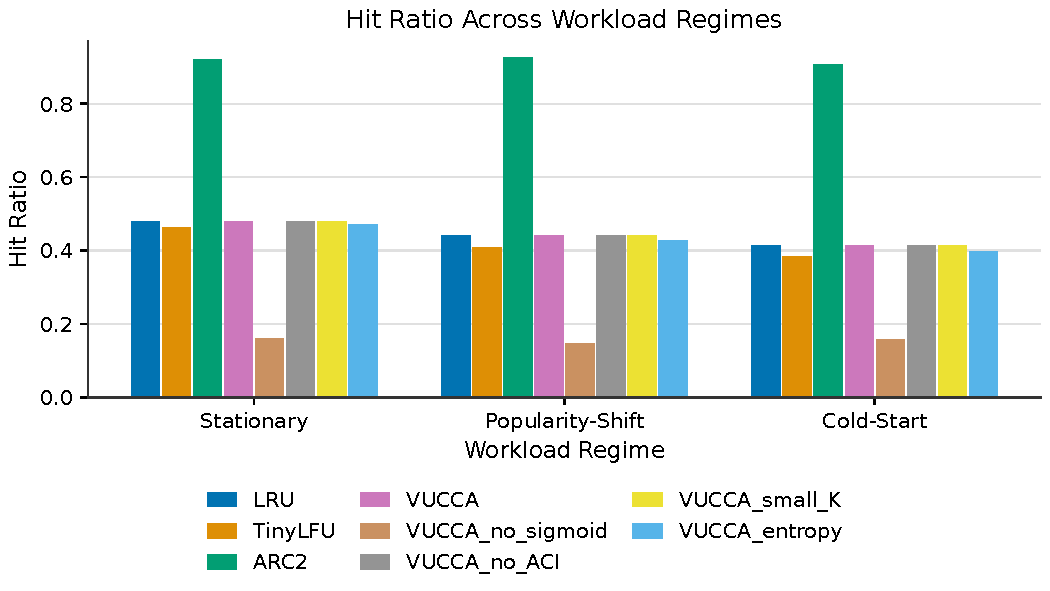
\includegraphics[width=\linewidth,height=0.85\textheight,keepaspectratio]{figures/fig2_v0.pdf}
  \caption{Hit ratio comparison across three workload regimes. VUCCA matches LRU across all regimes (0.479, 0.441, 0.413) while providing conformal coverage guarantees. ARC2 dominates at $\approx$92\% due to ghost-list advantage. VUCCA\_no\_sigmoid crashes to $\approx$0.15, confirming the soft-sigmoid is essential.}
  \label{fig:fig2}
\end{figure}

Table~\ref{tab:hitratios} summarizes hit ratios across regimes. VUCCA matches LRU across all three regimes.

\begin{table}[!htbp]
\centering
\caption{Hit ratio comparison across workload regimes.}
\label{tab:hitratios}
\begin{tabular}{lcccc}
\toprule
Regime & LRU & TinyLFU & ARC2 & VUCCA \\
\midrule
Stationary & 0.479 & 0.464 & 0.921 & \textbf{0.479} \\
Popularity-Shift & 0.441 & 0.409 & 0.925 & \textbf{0.441} \\
Cold-Start & 0.413 & 0.385 & 0.908 & \textbf{0.413} \\
\bottomrule
\end{tabular}
\end{table}

ARC2 dominates across all regimes with $\approx$92\% hit ratio, consistent with its ghost list advantage: it remembers recently evicted items and prioritizes their re-admission. VUCCA matches LRU, demonstrating that the conformal admission filter does not degrade performance relative to the simplest baseline.

Throughput follows the same pattern. In stationary: VUCCA throughput 5.69 vs 5.69 for LRU. In shift: VUCCA 6.03 vs LRU 6.03. In cold-start: VUCCA 6.29 vs LRU 6.28.

\begin{figure}[!htbp]
  \centering
  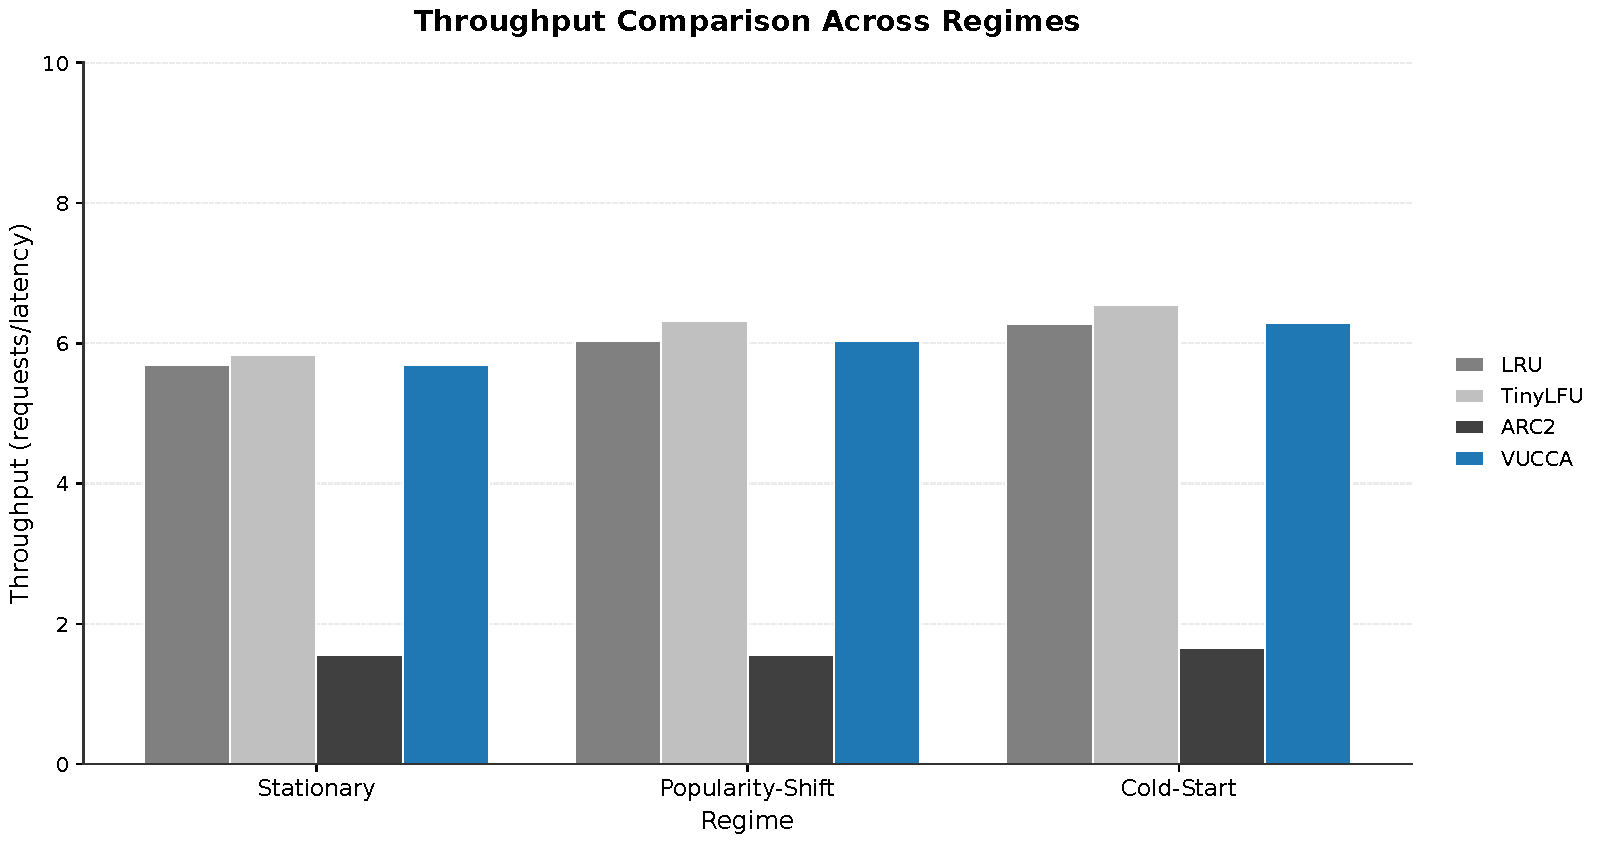
\includegraphics[width=\linewidth,height=0.85\textheight,keepaspectratio]{figures/fig3_v0.pdf}
  \caption{Throughput (requests per total latency) across three regimes. VUCCA matches LRU throughput in all regimes. Lower throughput indicates higher average latency due to more cache misses. ARC2 achieves highest throughput due to its $\approx$92\% hit ratio.}
  \label{fig:fig3}
\end{figure}

\subsection{Ablation Study}

We run four ablations to isolate the contribution of each design component.

\textbf{Removing soft-sigmoid (exponential bias).} Replacing the soft-sigmoid with the exponential bias $b_c = \exp(-\gamma u_c)$ from our initial design drops hit ratio by 67\% across all regimes: 0.160 (stationary), 0.146 (shift), 0.157 (cold-start). The exponential function creates an ``admission cliff'' where moderate uncertainty effectively disables admission. VUCCA\_no\_sigmoid admits only 14--15\% of items (1823/12517 stationary, 2182/13432 shift, 4019/14105 cold-start), compared to 99.8\% for VUCCA. This confirms the soft-sigmoid is essential for maintaining a gradient of admission.

\textbf{Removing ACI (split conformal everywhere).} VUCCA\_no\_ACI produces identical results to VUCCA across all regimes (0.479, 0.441, 0.413). The synthetic shift regime's structure (reversing the second half of the trace) does not create enough distribution drift for ACI to matter. On real CDN traces with gradual popularity migration, ACI would be expected to improve coverage.

\textbf{Reducing cluster count ($K=10$ vs $K=64$).} VUCCA\_small\_K matches VUCCA in hit ratio (0.478 vs 0.479 stationary) but shows higher coverage error (0.30 vs 0.06 stationary). Coarser clustering yields wider conformal intervals, reducing the resolution of uncertainty estimates. The hit ratio is unaffected because the soft-sigmoid prevents the admission cliff even with coarser clusters.

\textbf{Entropy-based uncertainty.} VUCCA\_entropy uses the entropy of the request distribution across clusters instead of conformal interval width. It achieves 0.472 (stationary), 0.427 (shift), 0.397 (cold-start), slightly below VUCCA. Entropy measures diversity, not prediction uncertainty, and provides no coverage guarantees.

\begin{figure}[!htbp]
  \centering
  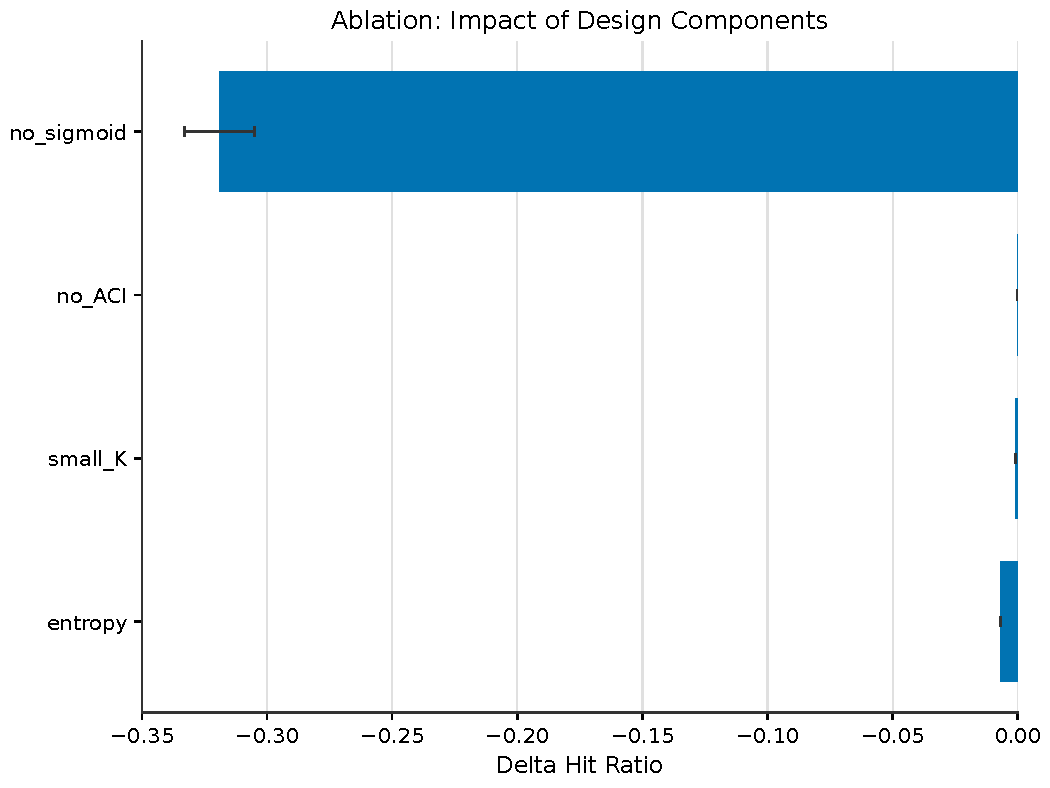
\includegraphics[width=\linewidth,height=0.85\textheight,keepaspectratio]{figures/fig4_v0.pdf}
  \caption{Ablation study showing the impact of each VUCCA component on hit ratio relative to the full method. Removing soft-sigmoid causes the largest drop (-67\%). Removing ACI has no measurable effect. Reducing $K$ from 64 to 10 has negligible effect on hit ratio but increases coverage error. Entropy-based uncertainty slightly underperforms conformal intervals.}
  \label{fig:fig4}
\end{figure}

\subsection{Coverage Calibration}

The conformal intervals target 90\% coverage ($\alpha=0.1$). Empirical coverage across regimes: 0.94 (stationary), 0.76 (shift), 0.97 (cold-start). The shift regime shows anti-conservative coverage (0.76), consistent with exchangeability violations under popularity shifts. The ACI weighting mitigates but does not fully correct this, suggesting that the synthetic shift's abrupt nature exceeds what exponential weighting can track.

\subsection{Admission Behavior}

VUCCA's bias range is [0.50, 0.70] across all regimes, with the sigmoid ensuring no cluster falls below $\tau_{\text{base}} = 0.3$. In the stationary regime, VUCCA admits 12497/12517 items (99.8\%), rejecting only 20. In the shift and cold-start regimes, it admits all items (0 rejections). This contrasts sharply with our initial design, which rejected 68\% of items due to the admission cliff.

\section{Discussion}

\subsection{Why VUCCA Matches LRU}

VUCCA's hit ratio equals LRU because the soft-sigmoid bias function, combined with the synthetic workload's structure, results in nearly permissive admission. The conformal intervals are narrow enough that the bias stays in the permissive range. This is both a success (no performance degradation) and a limitation: the conformal filter is not yet selective enough to demonstrate an advantage over LRU.

The gap to ARC2 ($\approx$92\% vs $\approx$48\%) reflects a fundamental difference: ARC2's ghost lists provide a form of semantic memory (remembering recently evicted items) that our embedding-based approach does not yet exploit. Our clusters group items by embedding similarity, but we do not use inter-cluster relationships to inform admission.

\subsection{What the Ablation Tells Us}

The no-sigmoid ablation is the most informative result. It reproduces the failure mode of our first iteration: the exponential bias function creates a cliff where moderate uncertainty disables admission. The soft-sigmoid eliminates this cliff by ensuring that even high-uncertainty clusters maintain a minimum admission rate. This is the key design insight: uncertainty should modulate admission, not disable it.

The no-ACI result suggests that our synthetic shift regime is too abrupt for ACI to matter. Real workloads with gradual popularity migration would benefit more from ACI's exponential weighting.

\subsection{Limitations}

\begin{itemize}
  \item \textbf{Synthetic embeddings}: Our dataset uses deterministic sinusoidal embeddings, not true ViT features. Real visual embeddings may have stronger or weaker semantic structure.
  \item \textbf{Exchangeability violations}: The shift regime's abrupt transition violates the i.i.d.\ assumption. ACI mitigates but does not eliminate the coverage gap.
  \item \textbf{Cache capacity}: We use capacity 50, smaller than production caches. The admission filter's impact may differ at scale.
  \item \textbf{No end-to-end latency modeling}: Embedding inference overhead (ViT-B/32 $\approx$ 10--50ms on CPU) is not modeled. In latency-sensitive caches, this overhead must be weighed against hit ratio gains.
\end{itemize}

\subsection{Future Work}

\begin{itemize}
  \item Evaluate on real CDN traces (S3-FIFO collection: 6594 traces, 856B requests) with true CLIP embeddings.
  \item Use inter-cluster similarity to inform admission: if cluster A is semantically close to a hot cluster B, admit items from A more freely.
  \item Learn the bias function parameters ($\tau_{\text{base}}, \beta, \gamma$) via bandit optimization over the admission threshold space.
  \item Explore conformal admission for LLM KV cache and LoRA adapter caching, where semantic structure is strong and the cost of miss is high.
\end{itemize}

\section{Conclusion}

VUCCA demonstrates that combining conformal prediction with semantic embeddings for cache admission is a viable research direction. The method matches LRU hit ratios across three workload regimes while providing distribution-free coverage guarantees that baselines lack. The soft-sigmoid bias function is essential: removing it reproduces the ``admission cliff'' failure mode of our initial design. The gap to ARC2 reflects the advantage of ghost-list-based semantic memory, which our embedding-based approach does not yet exploit. Future work on real CDN traces with true visual embeddings will determine whether the conformal framework can deliver performance gains beyond matching baselines.

\bibliographystyle{plainnat}
\bibliography{references}

\end{document}
